\chapter{Methodology}
\label{chap:methodology}

\lettrine[lines=3, findent=3pt, nindent=0pt]{C}{hapter} 3 deals with software and methodologies used for building the \gls{ids}. Starting with the concept behind the code, will then be discussed the scripts used, the pre-processing done to the chosen dataset, along with some statistics about the latter and the algorithms adopted in the \gls{ml} model training. In the final section will also be provided a \gls{poc} to demonstrate the functioning of the final product.

%----------------------------------------------------
% CONCEPT
%----------------------------------------------------

\section{Concept}
\label{sec:concept}

\textcolor{dimgray}{\lipsum[1]}

%----------------------------------------------------
% MODEL TRAINING
%----------------------------------------------------

\section{\gls{ml} Model Training}
\label{sec:model-training}

\textcolor{dimgray}{\lipsum[1]}

%----------------------------------------------------
% PRE-PROCESSING
%----------------------------------------------------

\subsection{Pre-Processing}
\label{subsec:pre-processing}

\textcolor{dimgray}{\lipsum[1]}

%----------------------------------------------------
% FEATURES AND STATISTICS
%----------------------------------------------------

\subsection{Features and Statistics}
\label{subsec:features-statistics}

\textcolor{dimgray}{\lipsum[1]}

\begin{figure}[h!]
    \centering
    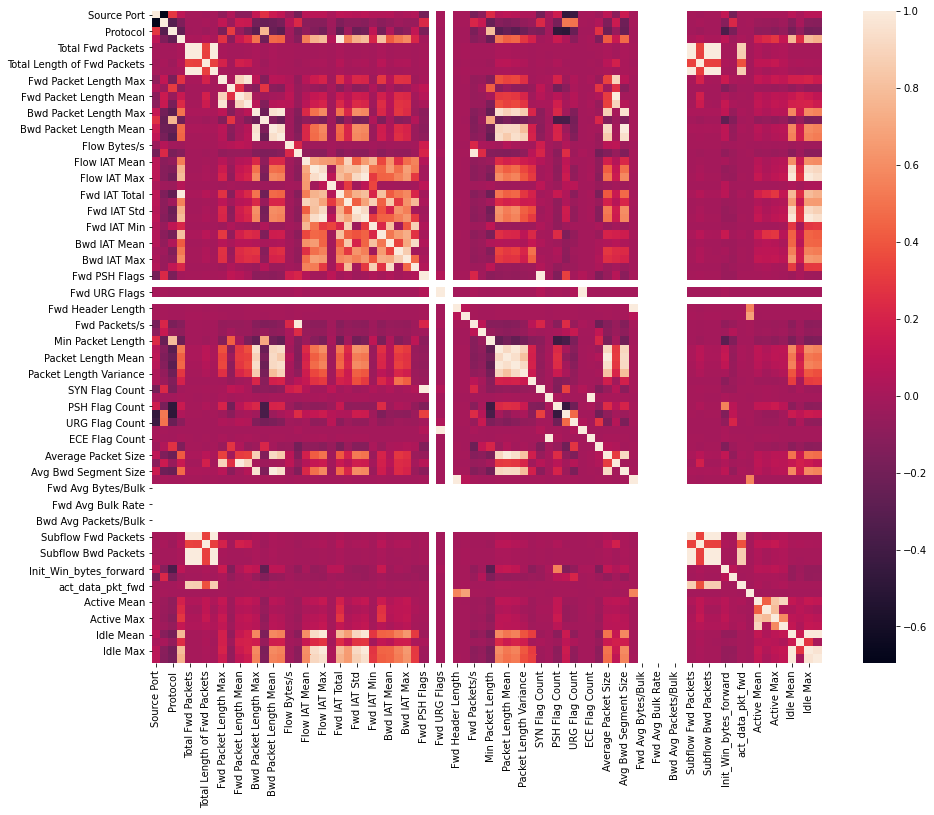
\includegraphics[scale=0.5]{assets/figures/chapter3/feature-correlation.png}
    \caption{Feature Correlation Matrix of CICIDS2017}
    \label{fig:feature-correlation}
\end{figure}

%----------------------------------------------------
% CLASSIFICATION
%----------------------------------------------------

\subsection{Classification}
\label{subsec:classification}

\textcolor{dimgray}{\lipsum[1]}

\begin{figure}[h!]
    \centering
    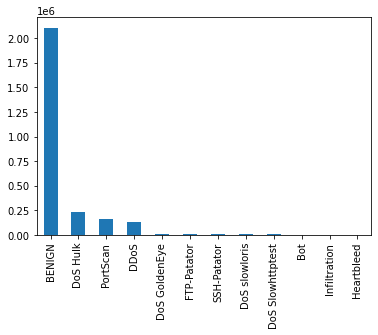
\includegraphics[scale=0.6]{assets/figures/chapter3/traffic_distribution.png}
    \caption{Traffic Distribution}
    \label{fig:traffic-distribution}
\end{figure}

%----------------------------------------------------
% NETWORK MONITOR
%----------------------------------------------------

\section{Network Monitor}
\label{sec:monitor-implementation}

\textcolor{dimgray}{\lipsum[1]}

%----------------------------------------------------
% ML INTEGRATION
%----------------------------------------------------

\subsection{\gls{ml} Integration}
\label{subsec:ml-integration}

\textcolor{dimgray}{\lipsum[1]}

\begin{figure}
    \begin{code}[colback=white]{Monitor.py}
if packet.getFwdID() in current_flows.keys():
flow = current_flows[packet.getFwdID()]

# check for timeout
# for some reason they only do it if packet count > 1
if (packet.getTimestamp() - flow.getFlowStartTime()) > FlowTimeout:
    classify(flow.terminated())
    del current_flows[packet.getFwdID()]
    flow = Flow(packet)
    current_flows[packet.getFwdID()] = flow

# check for fin flag
elif packet.getFINFlag() or packet.getRSTFlag():
    flow.new(packet, 'fwd')
    classify(flow.terminated())
    del current_flows[packet.getFwdID()]
    del flow
\end{code}
\end{figure}

\textcolor{dimgray}{\lipsum[1]}

%----------------------------------------------------
% MONITORING PIPELINE
%----------------------------------------------------

\subsection{Monitoring Pipeline}
\label{subsec:monitoring-pipeline}

\textcolor{dimgray}{\lipsum[1]}

%----------------------------------------------------
% POC
%----------------------------------------------------

\section{Proof of Concept}
\label{sec:poc}

\textcolor{dimgray}{\lipsum[1-10]}

%----------------------------------------------------
% TRAFFIC ACQUISITION
%----------------------------------------------------

\subsection{Traffic Acquisition}
\label{subsec:traffic-acquisition}

\textcolor{dimgray}{\lipsum}

%----------------------------------------------------
% TOPOLOGY
%----------------------------------------------------

\subsection{Topology}
\label{subsec:topology}

\textcolor{dimgray}{\lipsum}
